
\subsection{. Explain in detail how you implemented the circuit
breaker
.}

We have created a \textit{circuit-breaker} by using the Netflix Hystrix fault tolerance library. The application is a client for web services, and it is a middleware between web services and users. It can't be implemented directly on the user side. Otherwise, all users should prove it. It calls the web service with all URL options mentioned in the description of part 1. For every service of serviceapi, we have a fallback method. If the webservice is down then \textit{circuit-breaker} application will send the message that particular service is not working at the moment. You can see the design here in the diagram:

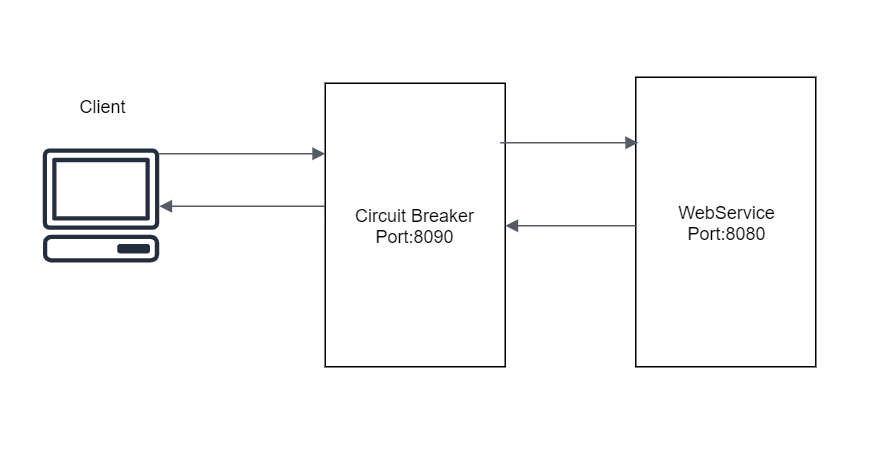
\includegraphics[keepaspectratio,width=0.8\textwidth,angle=0]{images/Circuit.PNG}

One can build the application:

\begin{itemize}
\item mvnw package
\end{itemize}

Then Execute:

\begin{itemize}

\item mvnw spring-boot:run

\end{itemize}
